\documentclass{article}
\usepackage[utf8]{inputenc}
\usepackage{graphicx}
\begin{document}
\section{Introduction}
The goal of this project is to analyze our Taxi dataset using multiple correspondence analysis using the FactorMineR library. This is similar to principal component analysis except it performs better for categorical data. We are mainly interested in finding the relationship between the \textit{Total\_amount} variable and a series of categorical variables we will investigate later.

\section{Data Description}
We are working with the Taxi Dataset from before. A Proposition from my last investigation involved dropping all erroneous rows before feature generation began. At this point we have 4566 rows. There are only two erroneous rows still in the dataset which have now been removed so we have 4564 rows. We also drop the missing values leaving 4433 rows.

\section{Data cleaning}
A script has been included from previous work on PCA to clean up the data.

\section{Data Preparation}
\subsection{Discretization Of Variables}
Next we need to convert The following into Discrete Variables:
\begin{enumerate}
\item Total\_amount
\item Trip\_distance
\item Fare\_amount
\end{enumerate}
We rename the quartiles for the above variables are set to Very Small, Small, Moderate, High.

The following need to be made into factors:
\begin{enumerate}
\item Extra
\item MTA\_tax
\item Tolls\_amount
\item improvement\_surcharge
\end{enumerate}

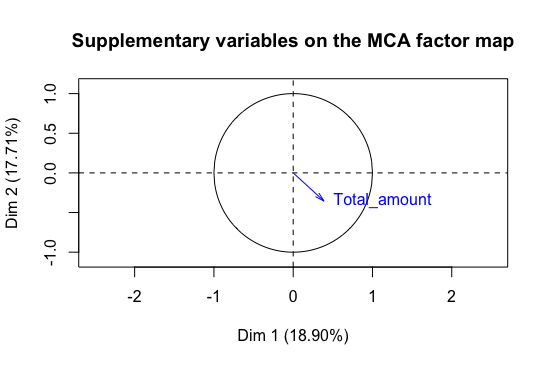
\includegraphics[width=\textwidth]{Rplot.png}

The below graphs show the most important and well represented values in our dataset which correlate with fare amounts.

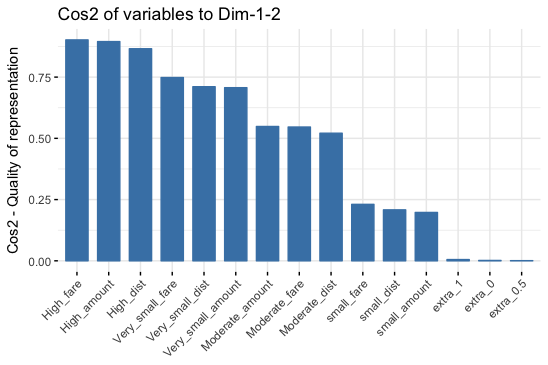
\includegraphics[width=\textwidth]{Cos2Dim.png}

\section{Contribution of Dimensions}
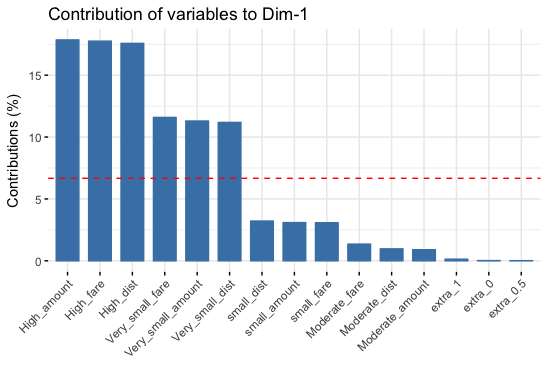
\includegraphics[width=\textwidth]{Dim1.png}
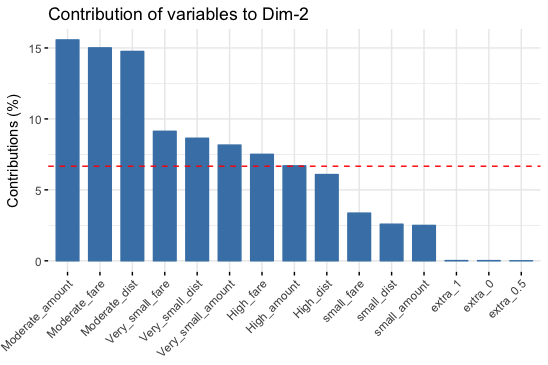
\includegraphics[width=\textwidth]{Dim2.png}

If a variable category is well represented by two dimensions, the sum of the cos2 is closed to one. For some of the row items, more than 2 dimensions are required to perfectly represent the data.

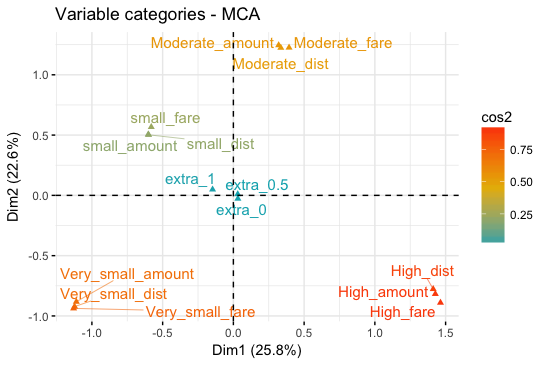
\includegraphics[width=\textwidth]{FViz.png}

\label{my-label}
\begin{tabular}{lll}
& R2 & p.value \\
Tamount\_inclass       & 0.940182014 & 0.000000e+00 \\
Trip\_distance\_inclass & 0.934443162 & 0.000000e+00 \\
Fare\_amount\_inclass   & 0.958139867 & 0.000000e+00 \\
Extra\_fac             & 0.004601991 & 3.654608e-05
\end{tabular}

The strongest weighting dimensions are Dim 1 and Dim 2. There are weighted as follows:

\label{my-label}
\begin{tabular}{llll}
& R2 & p.value \\
                       & Dim.1 & Dim.2 & Dim.3 \\
Tamount\_inclass        & 0.940 & 0.817 & 0.623 \\
Trip\_distance\_inclass  & 0.934 & 0.796 & 0.641 \\
Fare\_amount\_inclass    & 0.958 & 0.869 & 0.769 \\
Extra\_fac              & 0.005 & 0.001 & 0.000
\end{tabular}

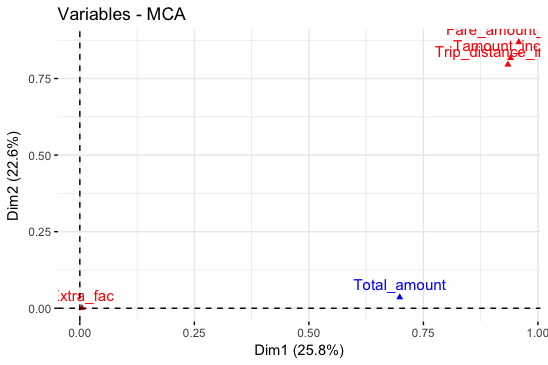
\includegraphics[width=\textwidth]{WeakExtra.png}
As you can see the Tax Amount, Trip distance and Fare Amount have large weightings in Dim 1 and Dim 2. Extra hardly correlates with these dimensions at all.


\section{Ellipse plots}
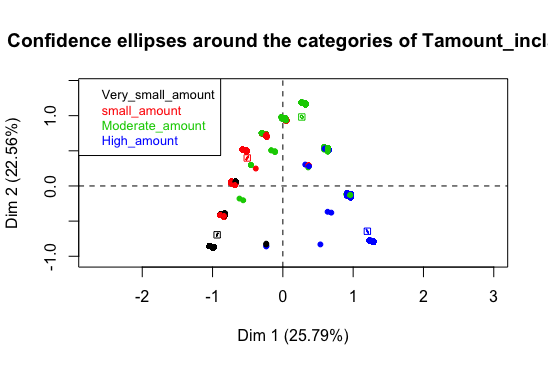
\includegraphics[width=\textwidth]{Tamount.png}
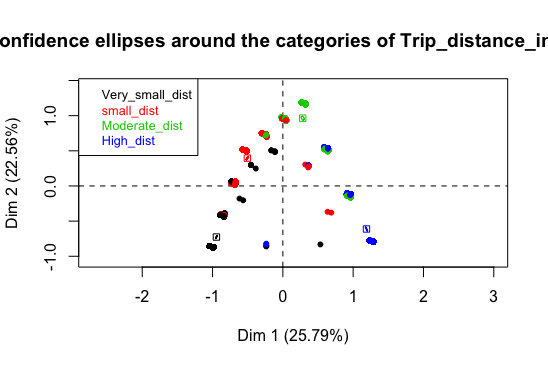
\includegraphics[width=\textwidth]{Trip_distance.png}
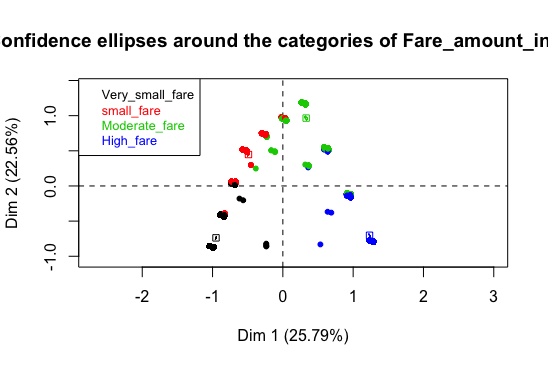
\includegraphics[width=\textwidth]{Fare_amount.png}
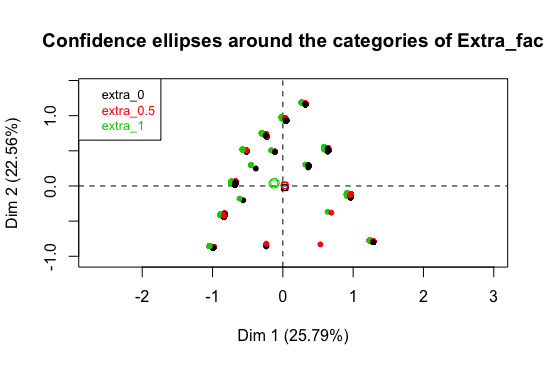
\includegraphics[width=\textwidth]{Extra_Fac.png}

\section{Analysis}
All graphs with the exception of the Extra graph seem to show a very clear clustering, while there is some overlap this is expected from the small set of possible outcomes.

The graph of Cos2 of the Variables in Dim 1 and 2 shows very clearly that High fare,amount and distance are all well represented by the dimensions chosen. Very small fares, amounts and distances are also well represented by these dimensions.

Dim 1 represents the High and Very small values well, meaning that there will be a large disparity in the horizontal axis of our plots. Dim 2 however represents Moderate values the most, so they should stand out in the vertical axis.

This again leaves Extra, as well as the small values as more difficult to distinguish, however they are still visually noticeable.
\end{document}
